
\section{Writing Yosys extensions in C++}

\begin{frame}
\sectionpage
\end{frame}

%%%%%%%%%%%%%%%%%%%%%%%%%%%%%%%%%%%%%%%%%%%%%%%%%%%%%%%%%%%%%%%%%%%%%%%%%%%%%

\subsection{Program Components and Data Formats}

\begin{frame}{\subsecname}
\begin{center}
\begin{tikzpicture}[scale=0.6, every node/.style={transform shape}]
	\tikzstyle{process} = [draw, fill=green!10, rectangle, minimum height=3em, minimum width=10em, node distance=15em]
	\tikzstyle{data} = [draw, fill=blue!10, ellipse, minimum height=3em, minimum width=7em, node distance=15em]
	\node[process] (vlog) {Verilog Frontend};
	\node[process, dashed, fill=green!5] (vhdl) [right of=vlog] {VHDL Frontend};
	\node[process] (ilang) [right of=vhdl] {Other Frontends};
	\node[data] (ast) [below of=vlog, node distance=5em, xshift=7.5em] {AST};
	\node[process] (astfe) [below of=ast, node distance=5em] {AST Frontend};
	\node[data] (rtlil) [below of=astfe, node distance=5em, xshift=7.5em] {RTLIL};
	\node[process] (pass) [right of=rtlil, node distance=5em, xshift=7.5em] {Passes};
	\node[process] (vlbe) [below of=rtlil, node distance=7em, xshift=-13em] {Verilog Backend};
	\node[process] (ilangbe) [below of=rtlil, node distance=7em, xshift=0em] {ILANG Backend};
	\node[process, fill=green!5] (otherbe) [below of=rtlil, node distance=7em, xshift=+13em] {Other Backends};

	\draw[-latex] (vlog) -- (ast);
	\draw[-latex] (vhdl) -- (ast);
	\draw[-latex] (ast) -- (astfe);
	\draw[-latex] (astfe) -- (rtlil);
	\draw[-latex] (ilang) -- (rtlil);
	\draw[latex-latex] (rtlil) -- (pass);
	\draw[-latex] (rtlil) -- (vlbe);
	\draw[-latex] (rtlil) -- (ilangbe);
	\draw[-latex] (rtlil) -- (otherbe);
\end{tikzpicture}
\end{center}
\end{frame}

%%%%%%%%%%%%%%%%%%%%%%%%%%%%%%%%%%%%%%%%%%%%%%%%%%%%%%%%%%%%%%%%%%%%%%%%%%%%%

\subsection{Simplified RTLIL Entity-Relationship Diagram}

\begin{frame}{\subsecname}
Between passses and frontends/backends the design is stored in Yosys' internal
RTLIL (RTL Intermediate Language) format. For writing Yosys extensions it is
key to understand this format.

\bigskip
\begin{center}
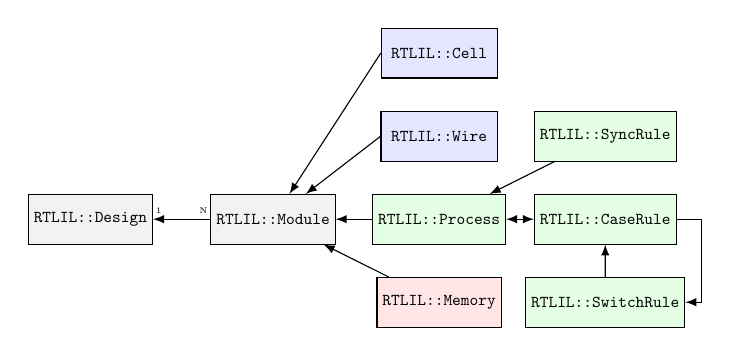
\begin{tikzpicture}[scale=0.6, every node/.style={transform shape}]
	\tikzstyle{entity} = [draw, fill=gray!10, rectangle, minimum height=3em, minimum width=7em, node distance=5em, font={\ttfamily}]
	\node[entity] (design) {RTLIL::Design};
	\node[entity] (module) [right of=design, node distance=11em] {RTLIL::Module} edge [-latex] node[above] {\tiny 1 \hskip3em N} (design);

	\node[entity] (process) [fill=green!10, right of=module, node distance=10em] {RTLIL::Process} (process.west) edge [-latex] (module);
	\node[entity] (memory) [fill=red!10, below of=process] {RTLIL::Memory} edge [-latex] (module);
	\node[entity] (wire) [fill=blue!10, above of=process] {RTLIL::Wire} (wire.west) edge [-latex] (module);
	\node[entity] (cell) [fill=blue!10, above of=wire] {RTLIL::Cell} (cell.west) edge [-latex] (module);

	\node[entity] (case) [fill=green!10, right of=process, node distance=10em] {RTLIL::CaseRule} edge [latex-latex] (process);
	\node[entity] (sync) [fill=green!10, above of=case] {RTLIL::SyncRule} edge [-latex] (process);
	\node[entity] (switch) [fill=green!10, below of=case] {RTLIL::SwitchRule} edge [-latex] (case);
	\draw[latex-] (switch.east) -- ++(1em,0) |- (case.east);
\end{tikzpicture}
\end{center}
\end{frame}

%%%%%%%%%%%%%%%%%%%%%%%%%%%%%%%%%%%%%%%%%%%%%%%%%%%%%%%%%%%%%%%%%%%%%%%%%%%%%

\subsection{RTLIL without memories and processes}

\begin{frame}[fragile]{\subsecname}
After the commands {\tt proc} and {\tt memory} (or {\tt memory -nomap}), we are
left with a much simpler version of RTLIL:

\begin{center}
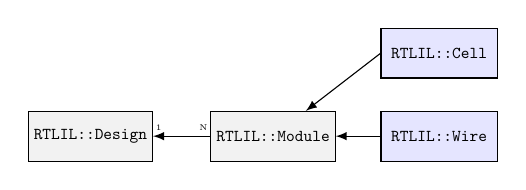
\begin{tikzpicture}[scale=0.6, every node/.style={transform shape}]
	\tikzstyle{entity} = [draw, fill=gray!10, rectangle, minimum height=3em, minimum width=7em, node distance=5em, font={\ttfamily}]
	\node[entity] (design) {RTLIL::Design};
	\node[entity] (module) [right of=design, node distance=11em] {RTLIL::Module} edge [-latex] node[above] {\tiny 1 \hskip3em N} (design);

	\node[entity] (wire) [fill=blue!10, right of=module, node distance=10em] {RTLIL::Wire} (wire.west) edge [-latex] (module);
	\node[entity] (cell) [fill=blue!10, above of=wire] {RTLIL::Cell} (cell.west) edge [-latex] (module);
\end{tikzpicture}
\end{center}

\bigskip
Many commands simply choose to only work on this simpler version:
\begin{lstlisting}[xleftmargin=0.5cm, basicstyle=\ttfamily\fontsize{8pt}{10pt}\selectfont]
for (RTLIL::Module *module : design->selected_modules() {
    if (module->has_memories_warn() || module->has_processes_warn())
        continue;
    ....
}
\end{lstlisting}

For simplicity we only discuss this version of RTLIL in this presentation.
\end{frame}

%%%%%%%%%%%%%%%%%%%%%%%%%%%%%%%%%%%%%%%%%%%%%%%%%%%%%%%%%%%%%%%%%%%%%%%%%%%%%

\subsection{Using dump and show commands}

\begin{frame}{\subsecname}
\begin{itemize}
\item The {\tt dump} command prints the design (or parts of it) in ILANG format. This is
a text representation of RTLIL.

\bigskip
\item The {\tt show} command visualizes how the components in the design are connected.
\end{itemize}

\bigskip
When trying to understand what a command does, create a small test case and
look at the output of {\tt dump} and {\tt show} before and after the command
has been executed.
\end{frame}

%%%%%%%%%%%%%%%%%%%%%%%%%%%%%%%%%%%%%%%%%%%%%%%%%%%%%%%%%%%%%%%%%%%%%%%%%%%%%

\subsection{The RTLIL Data Structures}

\begin{frame}{\subsecname}
The RTLIL data structures are simple structs utilizing {\tt pool<>} and
{\tt dict<>} containers (drop-in replacementments for {\tt
std::unordered\_set<>} and {\tt std::unordered\_map<>}).

\bigskip
\begin{itemize}
\item Most operations are performed directly on the RTLIL structs without
setter or getter functions.

\bigskip
\item In debug builds a consistency checker is run over the in-memory design
between commands to make sure that the RTLIL representation is intact.

\bigskip
\item Most RTLIL structs have helper methods that perform the most common operations.
\end{itemize}

\bigskip
See {\tt yosys/kernel/rtlil.h} for details.
\end{frame}

\subsubsection{RTLIL::IdString}

\begin{frame}{\subsubsecname}{}
{\tt RTLIL::IdString} in many ways behave like a {\tt std::string}. It is used
for names of RTLIL objects. Internally a RTLIL::IdString object is only a
single integer.

\medskip
The first character of a {\tt RTLIL::IdString} specifies if the name is {\it public\/} or {\it private\/}:

\medskip
\begin{itemize}
\item {\tt RTLIL::IdString[0] == '\textbackslash\textbackslash'}: \\
This is a public name. Usually this means it is a name that was declared in a Verilog file.

\bigskip
\item {\tt RTLIL::IdString[0] == '\$'}: \\
This is a private name. It was assigned by Yosys.
\end{itemize}

\bigskip
Use the {\tt NEW\_ID} macro to create a new unique private name.
\end{frame}

\subsubsection{RTLIL::Design and RTLIL::Module}

\begin{frame}[t, fragile]{\subsubsecname}
The {\tt RTLIL::Design} and {\tt RTLIL::Module} structs are the top-level RTLIL
data structures. Yosys always operates on one active design, but can hold many designs in memory.

\bigskip
\begin{lstlisting}[xleftmargin=1cm, basicstyle=\ttfamily\fontsize{8pt}{10pt}\selectfont, language=C++]
struct RTLIL::Design {
    dict<RTLIL::IdString, RTLIL::Module*> modules_;
    ...
};

struct RTLIL::Module {
    RTLIL::IdString name;
    dict<RTLIL::IdString, RTLIL::Wire*> wires_;
    dict<RTLIL::IdString, RTLIL::Cell*> cells_;
    std::vector<RTLIL::SigSig> connections_;
    ...
};
\end{lstlisting}

(Use the various accessor functions instead of directly working with the {\tt *\_} members.)
\end{frame}

\subsubsection{The RTLIL::Wire Structure}

\begin{frame}[t, fragile]{\subsubsecname}
Each wire in the design is represented by a {\tt RTLIL::Wire} struct:

\medskip
\begin{lstlisting}[xleftmargin=1cm, basicstyle=\ttfamily\fontsize{8pt}{10pt}\selectfont, language=C++]
struct RTLIL::Wire {
    RTLIL::IdString name;
    int width, start_offset, port_id;
    bool port_input, port_output;
    ...
};
\end{lstlisting}

\medskip
\hfil\begin{tabular}{p{3cm}l}
{\tt width} \dotfill & The total number of bits. E.g. 10 for {\tt [9:0]}. \\
{\tt start\_offset} \dotfill & The lowest bit index. E.g. 3 for {\tt [5:3]}. \\
{\tt port\_id} \dotfill & Zero for non-ports. Positive index for ports. \\
{\tt port\_input} \dotfill & True for {\tt input} and {\tt inout} ports. \\
{\tt port\_output} \dotfill & True for {\tt output} and {\tt inout} ports. \\
\end{tabular}
\end{frame}

\subsubsection{RTLIL::State and RTLIL::Const}

\begin{frame}[t, fragile]{\subsubsecname}
The {\tt RTLIL::State} enum represents a simple 1-bit logic level:

\smallskip
\begin{lstlisting}[xleftmargin=1cm, basicstyle=\ttfamily\fontsize{8pt}{10pt}\selectfont, language=C++]
enum RTLIL::State {
    S0 = 0,
    S1 = 1,
    Sx = 2, // undefined value or conflict
    Sz = 3, // high-impedance / not-connected
    Sa = 4, // don't care (used only in cases)
    Sm = 5  // marker (used internally by some passes)
};
\end{lstlisting}

\bigskip
The {\tt RTLIL::Const} struct represents a constant multi-bit value:

\smallskip
\begin{lstlisting}[xleftmargin=1cm, basicstyle=\ttfamily\fontsize{8pt}{10pt}\selectfont, language=C++]
struct RTLIL::Const {
    std::vector<RTLIL::State> bits;
    ...
};
\end{lstlisting}

\bigskip
Notice that Yosys is not using special {\tt VCC} or {\tt GND} driver cells to represent constants. Instead
constants are part of the RTLIL representation itself.
\end{frame}

\subsubsection{The RTLIL::SigSpec Structure}

\begin{frame}[t, fragile]{\subsubsecname}
The {\tt RTLIL::SigSpec} struct represents a signal vector. Each bit can either be a bit from a wire
or a constant value.

\bigskip
\begin{lstlisting}[xleftmargin=1cm, basicstyle=\ttfamily\fontsize{8pt}{10pt}\selectfont, language=C++]
struct RTLIL::SigBit
{
    RTLIL::Wire *wire;
    union {
        RTLIL::State data; // used if wire == NULL
        int offset;        // used if wire != NULL
    };
    ...
};

struct RTLIL::SigSpec {
    std::vector<RTLIL::SigBit> bits_; // LSB at index 0
    ...
};
\end{lstlisting}

\bigskip
The {\tt RTLIL::SigSpec} struct has a ton of additional helper methods to compare, analyze, and
manipulate instances of {\tt RTLIL::SigSpec}.
\end{frame}

\subsubsection{The RTLIL::Cell Structure}

\begin{frame}[t, fragile]{\subsubsecname (1/2)}
The {\tt RTLIL::Cell} struct represents an instance of a module or library cell.

\smallskip
The ports of the cell
are associated with {\tt RTLIL::SigSpec} instances and the parameters are associated with {\tt RTLIL::Const}
instances:

\bigskip
\begin{lstlisting}[xleftmargin=1cm, basicstyle=\ttfamily\fontsize{8pt}{10pt}\selectfont, language=C++]
struct RTLIL::Cell {
    RTLIL::IdString name, type;
    dict<RTLIL::IdString, RTLIL::SigSpec> connections_;
    dict<RTLIL::IdString, RTLIL::Const> parameters;
    ...
};
\end{lstlisting}

\bigskip
The {\tt type} may refer to another module in the same design, a cell name from a cell library, or a
cell name from the internal cell library:

\begin{lstlisting}[xleftmargin=1cm, basicstyle=\ttfamily\fontsize{6pt}{7pt}\selectfont]
$not $pos $neg $and $or $xor $xnor $reduce_and $reduce_or $reduce_xor $reduce_xnor
$reduce_bool $shl $shr $sshl $sshr $lt $le $eq $ne $eqx $nex $ge $gt $add $sub $mul $div $mod
$pow $logic_not $logic_and $logic_or $mux $pmux $slice $concat $lut $assert $sr $dff
$dffsr $adff $dlatch $dlatchsr $memrd $memwr $mem $fsm $_NOT_ $_AND_ $_OR_ $_XOR_ $_MUX_ $_SR_NN_
$_SR_NP_ $_SR_PN_ $_SR_PP_ $_DFF_N_ $_DFF_P_ $_DFF_NN0_ $_DFF_NN1_ $_DFF_NP0_ $_DFF_NP1_ $_DFF_PN0_
$_DFF_PN1_ $_DFF_PP0_ $_DFF_PP1_ $_DFFSR_NNN_ $_DFFSR_NNP_ $_DFFSR_NPN_ $_DFFSR_NPP_ $_DFFSR_PNN_
$_DFFSR_PNP_ $_DFFSR_PPN_ $_DFFSR_PPP_ $_DLATCH_N_ $_DLATCH_P_ $_DLATCHSR_NNN_ $_DLATCHSR_NNP_
$_DLATCHSR_NPN_ $_DLATCHSR_NPP_ $_DLATCHSR_PNN_ $_DLATCHSR_PNP_ $_DLATCHSR_PPN_ $_DLATCHSR_PPP_
\end{lstlisting}
\end{frame}

\begin{frame}[t, fragile]{\subsubsecname (2/2)}
Simulation models (i.e. {\it documentation\/} :-) for the internal cell library:

\smallskip
\hskip2em {\tt yosys/techlibs/common/simlib.v} and \\
\hskip2em {\tt yosys/techlibs/common/simcells.v}

\bigskip
The lower-case cell types (such as {\tt \$and}) are parameterized cells of variable
width. This so-called {\it RTL Cells\/} are the cells described in {\tt simlib.v}.

\bigskip
The upper-case cell types (such as {\tt \$\_AND\_}) are single-bit cells that are not
parameterized. This so-called {\it Internal Logic Gates} are the cells described
in {\tt simcells.v}.

\bigskip
The consistency checker also checks the interfaces to the internal cell library.
If you want to use private cell types for your own purposes, use the {\tt \$\_\_}-prefix
to avoid name collisions.
\end{frame}

\subsubsection{Connecting wires or constant drivers}

\begin{frame}[t, fragile]{\subsubsecname}
Additional connections between wires or between wires and constants are modelled using
{\tt RTLIL::Module::connections}:

\bigskip
\begin{lstlisting}[xleftmargin=1cm, basicstyle=\ttfamily\fontsize{8pt}{10pt}\selectfont, language=C++]
typedef std::pair<RTLIL::SigSpec, RTLIL::SigSpec> RTLIL::SigSig;

struct RTLIL::Module {
    ...
    std::vector<RTLIL::SigSig> connections_;
    ...
};
\end{lstlisting}

\bigskip
{\tt RTLIL::SigSig::first} is the driven signal and {\tt RTLIL::SigSig::second} is the driving signal.
Example usage (setting wire {\tt foo} to value {\tt 42}):
\begin{lstlisting}[xleftmargin=1cm, basicstyle=\ttfamily\fontsize{8pt}{10pt}\selectfont, language=C++]
module->connect(module->wire("\\foo"),
                RTLIL::SigSpec(42, module->wire("\\foo")->width));
\end{lstlisting}
\end{frame}

%%%%%%%%%%%%%%%%%%%%%%%%%%%%%%%%%%%%%%%%%%%%%%%%%%%%%%%%%%%%%%%%%%%%%%%%%%%%%

\subsection{Creating modules from scratch}

\begin{frame}[t, fragile]{\subsecname}
Let's create the following module using the RTLIL API:

\smallskip
\begin{lstlisting}[xleftmargin=1cm, basicstyle=\ttfamily\fontsize{8pt}{10pt}\selectfont, language=Verilog]
module absval(input signed [3:0] a, output [3:0] y);
    assign y = a[3] ? -a : a;
endmodule
\end{lstlisting}

\smallskip
\begin{lstlisting}[xleftmargin=1cm, basicstyle=\ttfamily\fontsize{8pt}{10pt}\selectfont, language=C++]
RTLIL::Module *module = new RTLIL::Module;
module->name = "\\absval";

RTLIL::Wire *a = module->addWire("\\a", 4);
a->port_input = true;
a->port_id = 1;

RTLIL::Wire *y = module->addWire("\\y", 4);
y->port_output = true;
y->port_id = 2;

RTLIL::Wire *a_inv = module->addWire(NEW_ID, 4);
module->addNeg(NEW_ID, a, a_inv, true);
module->addMux(NEW_ID, a, a_inv, RTLIL::SigSpec(a, 1, 3), y);

module->fixup_ports();
\end{lstlisting}
\end{frame}

%%%%%%%%%%%%%%%%%%%%%%%%%%%%%%%%%%%%%%%%%%%%%%%%%%%%%%%%%%%%%%%%%%%%%%%%%%%%%

\subsection{Modifying modules}

\begin{frame}{\subsecname}
Most commands modify existing modules, not create new ones.

When modifying existing modules, stick to the following DOs and DON'Ts:

\begin{itemize}
\item Do not remove wires. Simply disconnect them and let a successive {\tt clean} command worry about removing it.

\item Use {\tt module->fixup\_ports()} after changing the {\tt port\_*} properties of wires.

\item You can safely remove cells or change the {\tt connetions} property of a cell, but be careful when
changing the size of the {\tt SigSpec} connected to a cell port.

\item Use the {\tt SigMap} helper class (see next slide) when you need a unique handle for each signal bit.
\end{itemize}
\end{frame}

%%%%%%%%%%%%%%%%%%%%%%%%%%%%%%%%%%%%%%%%%%%%%%%%%%%%%%%%%%%%%%%%%%%%%%%%%%%%%

\subsection{Using the SigMap helper class}

\begin{frame}[t, fragile]{\subsecname}
Consider the following module:

\smallskip
\begin{lstlisting}[xleftmargin=1cm, basicstyle=\ttfamily\fontsize{8pt}{10pt}\selectfont, language=Verilog]
module test(input a, output x, y);
    assign x = a, y = a;
endmodule
\end{lstlisting}

In this case {\tt a}, {\tt x}, and {\tt y} are all different names for the same signal. However:

\smallskip
\begin{lstlisting}[xleftmargin=1cm, basicstyle=\ttfamily\fontsize{8pt}{10pt}\selectfont, language=C++]
RTLIL::SigSpec a(module->wire("\\a")), x(module->wire("\\x")),
                                       y(module->wire("\\y"));
log("%d %d %d\n", a == x, x == y, y == a); // will print "0 0 0"
\end{lstlisting}

The {\tt SigMap} helper class can be used to map all such aliasing signals to a
unique signal from the group (usually the wire that is directly driven by a cell or port).

\smallskip
\begin{lstlisting}[xleftmargin=1cm, basicstyle=\ttfamily\fontsize{8pt}{10pt}\selectfont, language=C++]
SigMap sigmap(module);
log("%d %d %d\n", sigmap(a) == sigmap(x), sigmap(x) == sigmap(y),
                  sigmap(y) == sigmap(a)); // will print "1 1 1"
\end{lstlisting}
\end{frame}

%%%%%%%%%%%%%%%%%%%%%%%%%%%%%%%%%%%%%%%%%%%%%%%%%%%%%%%%%%%%%%%%%%%%%%%%%%%%%

\subsection{Printing log messages}

\begin{frame}[t, fragile]{\subsecname}
The {\tt log()} function is a {\tt printf()}-like function that can be used to create log messages.

\medskip
Use {\tt log\_signal()} to create a C-string for a SigSpec object\footnote[frame]{The pointer returned
by {\tt log\_signal()} is automatically freed by the log framework at a later time.}:
\begin{lstlisting}[xleftmargin=1cm, basicstyle=\ttfamily\fontsize{8pt}{10pt}\selectfont, language=C++]
log("Mapped signal x: %s\n", log_signal(sigmap(x)));
\end{lstlisting}

\medskip
Use {\tt log\_id()} to create a C-string for an {\tt RTLIL::IdString}:
\begin{lstlisting}[xleftmargin=1cm, basicstyle=\ttfamily\fontsize{8pt}{10pt}\selectfont, language=C++]
log("Name of this module: %s\n", log_id(module->name));
\end{lstlisting}

\medskip
Use {\tt log\_header()} and {\tt log\_push()}/{\tt log\_pop()} to structure log messages:
\begin{lstlisting}[xleftmargin=1cm, basicstyle=\ttfamily\fontsize{8pt}{10pt}\selectfont, language=C++]
log_header("Doing important stuff!\n");
log_push();
for (int i = 0; i < 10; i++)
    log("Log message #%d.\n", i);
log_pop();
\end{lstlisting}
\end{frame}

%%%%%%%%%%%%%%%%%%%%%%%%%%%%%%%%%%%%%%%%%%%%%%%%%%%%%%%%%%%%%%%%%%%%%%%%%%%%%

\subsection{Error handling}

\begin{frame}[t, fragile]{\subsecname}
Use {\tt log\_error()} to report a non-recoverable error:

\medskip
\begin{lstlisting}[xleftmargin=1cm, basicstyle=\ttfamily\fontsize{8pt}{10pt}\selectfont, language=C++]
if (design->modules.count(module->name) != 0)
    log_error("A module with the name %s already exists!\n",
            RTLIL::id2cstr(module->name));
\end{lstlisting}

\bigskip
Use {\tt log\_cmd\_error()} to report a recoverable error:
\begin{lstlisting}[xleftmargin=1cm, basicstyle=\ttfamily\fontsize{8pt}{10pt}\selectfont, language=C++]
if (design->selection_stack.back().empty())
    log_cmd_error("This command can't operator on an empty selection!\n");
\end{lstlisting}

\bigskip
Use {\tt log\_assert()} and {\tt log\_abort()} instead of {\tt assert()} and {\tt abort()}.
\end{frame}

%%%%%%%%%%%%%%%%%%%%%%%%%%%%%%%%%%%%%%%%%%%%%%%%%%%%%%%%%%%%%%%%%%%%%%%%%%%%%

\subsection{Creating a command}

\begin{frame}[t, fragile]{\subsecname}
Simply create a global instance of a class derived from {\tt Pass} to create
a new yosys command:

\bigskip
\begin{lstlisting}[xleftmargin=1cm, basicstyle=\ttfamily\fontsize{8pt}{10pt}\selectfont, language=C++]
#include "kernel/yosys.h"
USING_YOSYS_NAMESPACE

struct MyPass : public Pass {
    MyPass() : Pass("my_cmd", "just a simple test") { }
    virtual void execute(std::vector<std::string> args, RTLIL::Design *design)
    {
        log("Arguments to my_cmd:\n");
        for (auto &arg : args)
            log("  %s\n", arg.c_str());

        log("Modules in current design:\n");
        for (auto mod : design->modules())
            log("  %s (%d wires, %d cells)\n", log_id(mod),
                    GetSize(mod->wires), GetSize(mod->cells));
    }
} MyPass;
\end{lstlisting}
\end{frame}

%%%%%%%%%%%%%%%%%%%%%%%%%%%%%%%%%%%%%%%%%%%%%%%%%%%%%%%%%%%%%%%%%%%%%%%%%%%%%

\subsection{Creating a plugin}

\begin{frame}[fragile]{\subsecname}
Yosys can be extended by adding additional C++ code to the Yosys code base, or
by loading plugins into Yosys.

\bigskip
Use the following command to compile a Yosys plugin:
\begin{lstlisting}[xleftmargin=1cm, basicstyle=\ttfamily\fontsize{8pt}{10pt}\selectfont]
yosys-config --exec --cxx --cxxflags --ldflags \
             -o my_cmd.so -shared my_cmd.cc --ldlibs
\end{lstlisting}

\bigskip
Or shorter:
\begin{lstlisting}[xleftmargin=1cm, basicstyle=\ttfamily\fontsize{8pt}{10pt}\selectfont]
yosys-config --build my_cmd.so my_cmd.cc
\end{lstlisting}

\bigskip
Load the plugin using the yosys {\tt -m} option:
\begin{lstlisting}[xleftmargin=1cm, basicstyle=\ttfamily\fontsize{8pt}{10pt}\selectfont]
yosys -m ./my_cmd.so -p 'my_cmd foo bar'
\end{lstlisting}
\end{frame}

%%%%%%%%%%%%%%%%%%%%%%%%%%%%%%%%%%%%%%%%%%%%%%%%%%%%%%%%%%%%%%%%%%%%%%%%%%%%%

\subsection{Summary}

\begin{frame}{\subsecname}
\begin{itemize}
\item Writing Yosys extensions is very straight-forward.
\item \dots and even simpler if you don't need RTLIL::Memory or RTLIL::Process objects.

\bigskip
\item Writing synthesis software? Consider learning the Yosys API and make your work
part of the Yosys framework.
\end{itemize}

\bigskip
\bigskip
\begin{center}
Questions?
\end{center}

\bigskip
\bigskip
\begin{center}
\url{http://www.clifford.at/yosys/}
\end{center}
\end{frame}

